%!TEX program = Traditional Builder with XeLaTeX
\documentclass[a4paper, zihao=-4, fontset = mac, oneside]{ctexbook} % 使文档按单面打印模式排版
% \usepackage[UTF8,scheme=chinese,heading]{ctex}

% math
\usepackage{amsmath, amsthm, amssymb} % Math
\usepackage{wasysym} % Greek alphabets
\usepackage{unicode-math} % Greek alphabets, 替换MnSymbol. NOTE: 但只能在xelatex或者lualatex中使用
\usepackage{mathrsfs, amsfonts} % Math fonts

% document
\usepackage{geometry} % Formatting
\usepackage{graphicx} % Required for inserting images
\usepackage{titlesec} % 定制章节标题样式
\usepackage{titletoc} % 定制目录格式
\usepackage{fancyhdr} % 引入fancyhdr宏包来控制页眉页脚
\usepackage{caption} % 定义caption
\usepackage{etoolbox} % 脚注通篇连续编号
\usepackage{listings} % 代码输入
\usepackage{hologo} % LaTeX logo支持
\usepackage{setspace} % 占位

% citation
\usepackage{hyperref} % 引用链接
\usepackage[
  backend=biber,
  style=gb7714-2005,
  citestyle=authoryear,
  sorting=nyvt,
  maxnames=1,
  minnames=1,
  maxbibnames=99,
  doi=false,
  gbpub=false]{biblatex}

% table
\usepackage{xcolor} % color
\usepackage{booktabs} % 使用booktabs表格形式
\usepackage{tabularx} % 在表格中制造换行
\usepackage{array} % 行间距

% font
\usepackage{fontspec, xeCJK} % 控制字体
\usepackage{anyfontsize} % 控制字体大小和行距

% ---------------------- 设置页面边距 ---------------------- 
\geometry{
  a4paper,
  top=3.5cm, 
  bottom=2.5cm, 
  left=2.5cm, 
  right=2.5cm,
  headheight=2.5cm,
  footskip=2cm,
  bindingoffset=0cm
  }
\setlength{\oddsidemargin}{0pt} % 奇数页左边距偏移
\setlength{\evensidemargin}{0pt} % 偶数页左边距偏移
% \geometry{top=1.5cm, bottom=1.5cm, left=5cm, right=1cm} % 开题报告版本


% ----------------------  标题与段落 ---------------------- 
% 设置中文模板的日期格式和摘要名称
\ctexset{
  today=big, % 日期格式为大写
  abstractname=简介 % 摘要名称设置为“简介”
}

% 设置chapter标题格式
\titleformat{\chapter}[block]
{\centering\zihao{3}\heiti} % 居中、三号、黑体
{\thechapter}
{1em}
{}
[\vspace{1ex}] % 段后空1行

% 设置chapter标题的前后间距
\titlespacing{\chapter}
{0pt} % 左边距
{1ex} % 段前空1行  
{1ex} % 段后空1行

% 重新定义section标题格式
\titleformat{\section}[hang]  % hang表示标题采用悬挂式样式
{\heiti\zihao{4}\raggedright}  % 黑体、四号、左对齐
{\thesection}{1em}{}  % 编号与标题间距1em

% 设置section标题的前后间距
\titlespacing{\section}
{0pt}  % 左边距
{1ex}  % 段前空1行
{1ex}  % 段后空1行

% 重新定义subsection标题格式
\titleformat{\subsection}[hang]  % hang表示标题采用悬挂式样式
{\heiti\zihao{-4}\raggedright}  % 黑体、小四号、左对齐
{\thesubsection}{1em}{}  % 编号与标题间距1em

% 设置subsection标题的前后间距
\titlespacing{\subsection}
{0pt}  % 左边距
{1ex}  % 段前空1行
{1ex}  % 段后空1行

% ----------------------  页眉、页码、脚注、锁进、行距 ---------------------- 
% 脚注通篇连续编号
\counterwithout{footnote}{chapter} 

% 修改脚注行距
\let\oldfootnote\footnote
\renewcommand{\footnote}[1]{%
  \oldfootnote{\setstretch{1.5}#1}% 设置脚注行距为 1.2 倍
}

% 添加首行缩进,两个字符
\usepackage{indentfirst}
\setlength{\parindent}{2em}

% 设置行距
\renewcommand{\baselinestretch}{1.0}
\setlength{\parskip}{0pt}
\linespread{1.5}  % 固定行距20磅约等于1.5倍行距

% 设置页眉样式
\pagestyle{fancy}
\fancyhf{} % 清空默认页眉页脚
\fancyhead[C]{\zihao{5} 浙江财经大学硕士毕业论文} % 设置字号与居中
\fancyfoot[C]{\thepage} % 居中显示页码

% ----------------------  设置字体 ---------------------- 
% 从本地创建字体命令
%\newfontfamily\mysongti[Path=./]{stsong.ttf}
%\newfontfamily\mykaiti[Path=./]{stkaiti.ttf}
%\newfontfamily\mykaitigb[Path=./]{kaiti_GB2312.ttf}
%\newfontfamily\myheiti[Path=./]{simhei.ttf}
%\newfontfamily\myxihei[Path=./]{stxihei.ttf}

\setCJKmainfont{简宋} % 设置默认中文字体为宋体
\setmainfont{Times New Roman} % 设置默认英文字体为Times New Roman
%\newfontfamily\kaiti{Kai}
\newfontfamily\kaitigb[Path=./]{楷体_GB2312.ttf}

% ------------------------ caption样式 ------------------------------
% 设置 caption 与 figure 之间的距离
\setlength{\abovecaptionskip}{11pt}
\setlength{\belowcaptionskip}{9pt}

% 设置表格的 caption 与 table 之间的垂直距离
\captionsetup[table]{skip=2pt}

% 设置图片的 caption 格式
\renewcommand{\thefigure}{\thechapter-\arabic{figure}}
\captionsetup[figure]{font=small,labelsep=space}

% 设置表格的 caption 格式
\renewcommand{\thetable}{\thechapter-\arabic{table}}
\captionsetup[table]{font=small,labelsep=space}

% ----------------------  宏包设置 ---------------------- 
% hyperref设置
\hypersetup{
  pdflang = zh-CN, % 设置PDF文档语言为简体中文
  pdftitle = {浙江财经大学学位论文-李晨逸}, % PDF标题
  pdfauthor = {Suicidal Bumblebee} % 作者
}%

% array调整表格行间距
\renewcommand{\arraystretch}{1.5}

% citation
\ExecuteBibliographyOptions{sortlocale=zh__pinyin} % 设置排序语言环境为中文拼音
\addbibresource{Papers.bib} % 添加文献bib文件
\DeclareSourcemap{
  \maps[datatype=bibtex]{
    \map{
      \step[fieldset=url, null] % 删除 url 字段
    }
    \map{
      \step[fieldset=librarycatalog, null] % 删除 librarycatalog 字段
    }
  }
}

\begin{document}

\frontmatter

\mainmatter
% ---------------------------------------- 文献综述 ----------------------------------------
\chapter*{文献综述}

劳动力流动作为经济社会发展的重要表征,其研究要点在于提供合适的方法和寻找符合现实逻辑的影响因素。本文通过系统梳理国内外近几十年来的经典文献与前沿成果,试图厘清学术脉络的演进逻辑,为后续实证研究提供标准。
在研究方法层面,现有文献呈现出从静态分析向动态追踪的范式转变。就影响因素而言,学者们已逐步突破传统经济变量的单一解释,将制度约束、社会网络、文化认同等非经济维度纳入分析体系。


\section{相关概念梳理}
劳动力回流是指原先从一个地区迁出的劳动力再次返回原籍地的现象。这种迁移可被视为可撤回的(retractable)或短暂的(temporary),与传统静态迁移模型所假设的单向永久性迁移存在显著差异。

劳动力回流研究具有以下特点:首先,从历史维度看,它是一个相对较新的现象,在人类工业化历程中出现较晚;其次,它挑战了传统人口迁移理论中从欠发达地区向发达地区单向流动的基本假设;再次,对于后发工业化国家而言,这一现象具有重要的政策意义。

在传统经济理论框架下,当目标地经济衰退导致预期收益低于原籍地时,返迁决策符合理性选择理论;然而当目标地仍能提供显著收入溢价时,劳动力选择返迁则构成理论悖论。这一现象值得深入研究,特别是对于后发工业化国家而言。

\textcite{CaiFangHuJiZhiDuYuLaoDongLiShiChangBaoHu2001}等学者指出,后发国家通常采取非均衡发展战略,通过制度化的城乡二元结构形成工农产品价格剪刀差,实现资源从传统农业部门向现代工业部门的系统性转移。这种情况下,劳动力回流可能不利于资本深化与工业化进程。
中国的工业化路径具有特殊性,融合了社会主义国家计划经济与市场经济转型的特点。20世纪50至80年代,由于资源稀缺,我国建立了以户籍制度为核心的空间资源配置体系,将有限资本集中于少数城市,形成公共服务的高度集聚。改革开放后,我国借鉴东亚发展型国家经验,采取出口导向型发展战略,特别是2001年加入世贸组织后,充分发挥人口红利的比较优势。\textcite{LinYiFuZhongGuoDeJingJiFaZhanZhanLueYuDiQuShouRuChaiJu2003}为这一发展路径提供了系统的理论支撑。
在快速工业化进程中,大量人口涌入城市,形成了沿海发达地区持续吸纳内陆剩余劳动力的迁移格局。然而,我国劳动力市场中却出现明显的回流现象,即农村居民进城打工后又返回原籍,形成农民工返潮现象。这一现象与后发国家工业化进程中的劳动力配置目标存在理论上的背离。

多项研究表明,户籍制度障碍可能是影响劳动力定居的首要因素。\textcite{RenYuanChengShiLiuDongRenKouDeSheHuiRongHeWenXianShuPing2006}指出,以户籍制度为依托的流动人口管理制度及相关社会福利制度对流动人口的限制与排斥对其社会融合有根本性影响。\textcite{LuYiLongHuKouHuanQiZuoYongMaHuJiZhiDuYuSheHuiFenCengHeLiuDong2008}认为即使经历了深刻改革,户籍制度仍然对劳动力自由流动造成客观阻碍,制约经济高质量发展。
另一种观点认为,源于1994年分税制改革的土地财政模式可能是劳动力回流的重要原因。\textcite{ChenYingFangNongMinGongZhiDuAnPaiYuShenFenRenTong2005}、\textcite{niehuihuaZhongguogaofangjiadexinzhengzhijingjixuejieshiYiZhengqihemou2013}及\textcite{YuJianXingDiFangFaZhanXingZhengFuDeXingWeiLuoJiJiZhiDuJiChu2012}等研究认为,土地出让金作为地方政府重要财源,导致政府维持较高地价,推高房价,增加城市居民住房负担,从而影响劳动力的定居决策。

除户籍与土地财政外,影响劳动力回流的因素还可能包括原籍地经济发展与就业机会增加、工资差距缩小、生活成本差异变化;家庭纽带与社会融入因素;以及公共服务可及性、返乡创业政策等制度因素。
综合来看,劳动力回流问题涉及多种制度与市场机制的交互作用。传统的线性迁移模型难以解释复杂现实情况,需引入更具动态性和多维视角的方法进行深入研究。
接下来对劳动力流动研究的主要方法进行梳理,以期为本研究提供合适的方法论支持。


\section{空间均衡方法}

根据\textcite{jiaEconomicsInternalMigration2023}的研究,劳动力迁移问题可采用两种研究方法,其中一种是空间均衡方法。该方法以迁移后形成的新空间一般均衡为核心,主要关注人口流动如何影响本地工资、区域房价等变量的市场出清。

空间均衡概念可追溯至20世纪中叶,\textcite{samuelsonSpatialPriceEquilibrium1952}提出的"空间价格均衡"框架考虑了运输成本对不同地点价格的影响,奠定了空间经济学基础。\textcite{tieboutPureTheoryLocal1956}提出"用脚投票"理论,假设消费者在无迁移成本和信息完全的条件下,会自由选择最能满足其偏好的社区。\textcite{harrisMigrationUnemploymentDevelopment1970}则构建了研究农村到城市迁移的两部门内部贸易模型,探讨了城乡工资差异的均衡状态。

受城市经济学发展影响,20世纪60-70年代,\textcite{alonsoLocationLandUse1964}、\textcite{muthCitiesHousingSpatial1969}和\textcite{millsAggregativeModelResource1967}开创的单中心城市模型考察了城市内部空间结构,为城市间移民研究奠定基础。\textcite{rosenHedonicPricesImplicit1974}提出的享乐定价模型能够通过观察特定地点便利设施对工资和租金的影响来量化这些设施的价值,为移民研究提供了重要工具。
基于Rosen模型,\textcite{robackWagesRentsQuality1982}正式确立了移民空间均衡模型,该模型假设个人会迁移至效用最高的地点,同时考虑金钱因素(工资、租金)和非金钱因素(便利设施)。在均衡状态下,工资和租金会调整以平衡不同地点的效用,使得没有人能通过迁移提高效用。这一模型成为理解便利设施如何影响移民模式和城市增长的基础框架。

20世纪80-90年代,空间均衡方法进一步扩展,纳入了住房市场动态、非贸易商品和异质性主体等因素。\textcite{glaeserWealthCitiesAgglomeration2009}强调住房供应弹性在决定城市成功表现(人口增长或收入增长)方面的关键作用。\textcite{morettiLocalLaborMarkets2011}提出了假设工人流动性有限且住房供应非固定的一般均衡模型,更贴近现实情况。\textcite{diamondDeterminantsWelfareImplications2016}构建了结构性空间均衡模型,研究技能分类增加的原因及其福利影响,考虑了偏好和技能的异质性。\textcite{coen-piraniEffectHouseholdAppliances2010}则开发了动态一般均衡模型,强调个体异质性在迁移决策中的作用。
近二十年来,空间均衡方法整合到定量空间经济学中,\textcite{ahlfeldtEconomicsDensityEvidence2015}和\textcite{reddingQuantitativeSpatialEconomics2017}扩展了Rosen-Roback框架,引入市场准入项,提供了内生价格作为基本面和地理因素函数的对数线性方程,更好地捕捉现代经济复杂性。\textcite{glaeserHousingDynamicsUrban2014}构建了动态的、线性的、理性的一般均衡模型,与住房市场典型事实相一致。\textcite{albertImmigrationSpatialEquilibrium2022}则将该方法应用于国际移民研究,记录了移民如何受原籍国支出影响而选择生活成本高昂的城市。


表格\ref{tab:_history of spatial equilibrium on migratory problem}概述了空间均衡方法在移民研究中的发展历程。

\begin{table}[!ht]
\centering
\caption{使用空间均衡方法研究人口流动的历史}
\label{tab:_history of spatial equilibrium on migratory problem}
\begin{tabularx}{\textwidth}{@{}lX@{}}
\toprule
\textbf{时期} & \textbf{关键发展}\\
\midrule
\textbf{1950年代} & \textcite{samuelsonSpatialPriceEquilibrium1952}引入了空间价格均衡,通过运输成本平衡不同地点的供需。奠定了空间均衡经济学的基础,但最初侧重于商品市场。\\
\textbf{1960-1970年代} & \textcite{muthCitiesHousingSpatial1969}和\textcite{millsAggregativeModelResource1967}开发了关注通勤和住房选择的城市内模型,影响了城际移民研究。为区位选择提供了空间框架,为移民应用奠定了基础。\\
\textbf{1970年代} & \textcite{rosenHedonicPricesImplicit1974}建立了享乐定价模型,通过工资和租金等观察到的价格来评估区位属性(例如便利设施),能够量化区位选择中的非金钱因素,为移民研究奠定了基础。 \\
\textbf{1980年代} & \textcite{robackWagesRentsAmenities1988}正式建立了一个一般均衡模型,其中工资、租金和便利设施使不同地点的效用均衡,从而解释了移民模式。成为研究移民的基石,将经济激励与区位决策联系起来。\\
\textbf{1980-1990年代} & \textcite{glaeserWealthCitiesAgglomeration2009}将住房供应弹性、非贸易商品和异质性主体纳入模型。通过解决住房动态和不同的移民偏好增强了现实性。\\
\textbf{2010年代} & \cite{reddingQuantitativeSpatialEconomics2017}整合市场准入和贸易成本,扩展 Rosen-Roback 模型,使用对数线性方程对工资和人口进行建模。改进了基础设施和贸易对移民影响的政策分析。\\
\textbf{近期} & 拓展:国际移民、信息约束、多部门和异构代理模型 \\
\bottomrule
\end{tabularx}
\end{table}

国内学者也运用空间均衡模型研究人口流动问题。\textcite{LiangRuoBingDiFangGongGongPinGongGeiZhongDeTieboutMoXingJiYuZhongGuoChengShiFangJieDeJingYanYanJiu2008}基于Tiebout模型验证了中国城市住房价格与地方公共品供给关系。\textcite{LiuHuaRenLiZiBenKongJianPeiZhiDeSheHuiFuLiXiaoYingYanJiuJiYuLiangHuaKongJianYiBanJunHengMoXingDeFenXi2024}构建了包含异质性劳动力生产率溢出和公共服务溢出的空间一般均衡模型,分析了人力资本空间配置优化的社会福利效应。\textcite{WangLiLiWoGuoRenKouQianYiChengBenChengShiGuiMoYuShengChanLu2020}结合空间均衡模型与地级市数据研究人口迁移对劳动力资源配置的影响。\textcite{WangLiLiTuDiGongGeiFangJieYuLaoDongLiKongJianPeiZhiXiaoLu2023}分析了土地供给政策对劳动力空间配置效率的影响,指出政府对建设用地指标的管控决定住房供给弹性,东部大城市的严格规制阻碍了人口向高生产率地区转移。\textcite{ZhaoFangZhongGuoChengShiHuaFaZhanJiYuKongJianJunHengMoXingDeYanJiu2017}基于\textcite{diamondDeterminantsWelfareImplications2016}的模型研究中国劳动力迁移机制,发现工资水平仍是主要影响因素,但城市舒适度对流动人口也具有重要作用。

尽管空间均衡方法影响深远,但其完全流动性和同质主体等假设过于简化了现实复杂性,对均衡条件的依赖也难以充分捕捉短期迁移动态或社会网络和文化因素的作用。此外,该方法在宏观层面有效,但难以解释微观个体行为,需要非均衡方法作为补充。这些局限性促使研究者发展更加细致的微观视角方法,以更好地理解劳动力迁移决策过程。


\section{个体微观视角与动态选择方法}

与空间均衡方法所关注的宏观均衡不同,个体微观视角研究方法着重于分析单个经济主体的决策过程。这种方法类似于交通道路模拟中的元胞自动机微观方法,而空间均衡则对应于流体力学宏观方法。

个体视角的劳动力流动研究始于\textcite{sjaastadCostsReturnsHuman1962}。Sjaastad提出了一个模型,假设个人根据迁移的成本和预期回报做出地点决策。这种观点将移民视为投资行为,强调了移民决策的动态特性。从生命周期角度看,个人决策(如储蓄、教育、婚姻)与移民选择相互关联,构成了一个统一的决策框架。\textcite{mincerFamilyMigrationDecisions1978}进一步发展了这一理论,考虑了家庭联合决策的情况,认识到家庭最优地点选择可能与个体配偶的最优选择存在差异。
\textcite{kennanEffectExpectedIncome2011}提出的个人移民选择模型是这一领域的重要发展。该模型允许个体技能、位置偏好和迁移成本的异质性,并将移民决策作为最优搜索过程处理,假设个人在扣除迁移成本后最大化预期终身收入。该研究的重要贡献在于将动态离散选择模型引入移民问题研究。

动态离散选择(Dynamic Discrete Choice, DDC)模型是研究个体或家庭如何在多个潜在居住地之间做出最优选择的理论框架,适用于分析人口迁移、城市发展和住房市场动态。DDC模型具有以下特征:离散时间序列的动态性;单个决策者面临有限且离散的选择集;选择持续存在;马尔可夫决策过程;随机决策环境;基于微观数据的显示偏好。这些特征使DDC成为研究动态迁移决策过程的理想工具,特别适合分析可撤回的迁移行为。

离散选择模型的理论源头可追溯至\textcite{thurstoneLawComparativeJudgment1927}提出的比较判定定律,该定律从心理激励角度解释了选择行为。\textcite{marschakBinarychoiceConstraintsRandom1960}将这种感知刺激解释为效用,提出了随机效用最大化(Random Utility Maximization, RUM)模型,奠定了现代离散选择模型的理论基础。\textcite{mcfaddenConditionalLogitAnalysis1973}则将二元逻辑模型扩展为条件逻辑模型,使其适用于多种选择情境。

动态离散选择模型的发展与动态规划理论密切相关。\textcite{bellmanDynamicProgramming1957}提出的动态规划为序列决策问题提供了数学框架,而\textcite{blackwellDiscreteDynamicProgramming1962}则为马尔可夫决策过程(Markov Decision Process, MDP)建立了理论基础。
经济学中的DDC模型研究始于20世纪80年代中期。\textcite{rustOptimalReplacementGMC1987}被视为该领域的开创性工作,提出了嵌套不动点(Nested Fixed Points, NFXP)算法进行最大似然估计。\textcite{ecksteinDynamicLabourForce1989}在此基础上构建了已婚女性劳动力参与率和生育率的动态模型,考虑了工作经验对工资的影响。\textcite{keaneStructuralEstimationBehavioral2011}系统介绍了离散选择动态规划(DCDP)模型的结构估计方法及其在劳动经济学中的应用。

由于DDC模型计算量巨大,\textcite{hotzConditionalChoiceProbabilities1993}提出了条件选择概率方法,避免了反复求解完整动态规划问题的需要。近年来,\textcite{suConstrainedOptimizationApproaches2012}提出的带均衡约束的数学规划(MPEC)进一步减轻了计算负担。表格\ref{tab:不同作者对于动态离散选择模型的贡献}总结了DDC模型方法论的关键发展。

\begin{table}[!ht]
\centering
\caption{不同作者对于动态离散选择模型的贡献}
\label{tab:不同作者对于动态离散选择模型的贡献}
\begin{tabularx}{\textwidth}{@{}cXX@{}} 
\toprule
\textbf{年份} & \textbf{作者} & \textbf{贡献}\\
\midrule
1987年 &John Rust &开发了嵌套不动点算法,提出经典的公交车发动机更换模型。\\
1993年 &V. Joseph Hotz、Robert A. Miller &开发了条件选择概率,作为领先的非解估计方法。\\
2012年 &Che-Lin Su、Kenneth Judd &提出带均衡约束的数学规划方法进行估计。\\
\bottomrule
\end{tabularx}
\end{table}

近年来,研究重点转向融入更为现实的行为假设并拓展应用领域。\textcite{utaraDynamicDiscreteChoice2024}探讨了动态不一致性问题,\textcite{heckmanDynamicDiscreteChoice2007}将动态选择模型与处理效应估计相结合,增强了政策分析能力。计算能力的进步使高维状态和多智能体模型成为可能,推动了该方法在卫生经济学、环境经济学和市场营销等领域的应用。

如\textcite{jiaEconomicsInternalMigration2023}所述,使用DDC模型探究劳动力迁移问题本质上是一种非均衡方法,与空间均衡方法形成鲜明对比。两者代表了不同的分析范式:空间均衡方法基于新古典经济学的一般均衡理论,强调区域间要素调整与市场出清,其研究视角聚焦于城市或区域层面的整体均衡状态。该方法通常假设劳动力具有同质性或有限异质性,在计量分析中多采用结构方程估计或联立方程系统,依赖区域层面的汇总数据,典型应用包括区域经济收敛性研究以及税收与公共服务的政策分析。
与之相对,基于DDC的最优居住地选择模型则以微观经济学的效用最大化理论为基础,关注个体或家庭在异质性偏好下的决策过程。该方法明确建模个体差异性和偏好多样性,在实证层面主要采用离散选择模型(如条件Logit、嵌套Logit等),并需要微观个体数据作为支撑。其典型应用场景涵盖农民工市民化决策、高技能人才流动等侧重微观行为机制的研究领域。两种方法在理论基础、分析视角、异质性处理、计量工具及数据需求等方面均存在系统性差异,分别体现了宏观均衡框架与微观决策逻辑的学术分野。

对于劳动力回流这一具有暂时性迁移特征的研究问题,微观方法提供了更为适合的分析框架。通过动态离散选择模型构建最优居住地序列选择模型,可以有效捕捉个体在不同时期的迁移决策及其影响因素。

\section{对回流迁移的研究}

通常进行科学研究时会强调国内与国外文献的融合,但在劳动力回迁问题上,国内国外在具体议题上存在较大不同。具体而言,在我国独特国情下,劳动力回流问题指的都是农民工返潮现象,而国外研究大致都是研究在一个自由流动的背景下劳动力如何自由选择的。在这个前提下,我们有必要先对国内外的学术工作分开进行总结,接着再从国外文献的研究方法中汲取有用的共性以服务于国内研究课题。

国外关于劳动力回流(return migration)的研究重点关注自由流动背景下个体和家庭如何在不同地点间进行迁移决策。与我国不同,国外研究通常聚焦于国际移民的往返迁移、临时性迁移及其经济和社会驱动因素。

早期研究如\textcite{gmelchReturnMigration1980}综合了南欧、东欧和加勒比地区的案例,指出20世纪初欧洲移民中有四分之一返回原籍国。
\textcite{wymanRoundtripAmericaImmigrants1993}则通过历史记载分析了1880-1930年间从美国返回欧洲的移民,归因于怀旧情绪和本土主义怨恨等因素。这些研究奠定了对回流迁移现象的基本理解。

\textcite{sjaastadCostsReturnsHuman1962}首次将移民定义为一种人力资本投资,强调个人在预期回报超过成本时选择迁移。这一静态框架为后续研究提供了基础,但其局限性在于无法处理多目的地选择问题。\textcite{tunaliRationalityMigration2000}尝试扩展至动态框架,但仍局限于二元选择。
\textcite{dierxLifecycleModelRepeat1988}则结合面板数据,分析家庭人力资本分布对迁移决策的影响,弥补了单期模型的不足。
\textcite{dahlMobilityReturnEducation2002} 通过罗伊模型探讨了自我选择迁移机制,解释了美国劳动者高流动性与地区教育回报差异之间的关系。\textcite{gemiciFamilyMigrationLabor2007}进一步构建包含家庭内部协商的动态模型,发现家庭纽带会抑制人口流动性并减缓工资增长。
在以上早期模型的基础上,\textcite{kennanEffectExpectedIncome2011}他们利用全国青年纵向调查(NLSY)中针对高中教育白人男性的面板数据,开发了一个动态离散选择模型,该模型允许在多个备选方案中进行最优的地点决策序列。该模型通过考虑收入前景来捕捉回归移民,发现地域工资差异和对更佳地点匹配的追求会影响决策,包括在当前收入不利的情况下回归。这标志着一项重大进展。
在这之后,
\textcite{dustmannEconomicsTemporaryMigrations2016}强调了临时迁移的重要性,提出一个通用理论框架,分析技能积累、技能回报率差异及消费偏好如何驱动跨国往返迁移。研究表明,即使缺乏外生冲击,这些内生机制仍能引致回流行为。\textcite{venatorDualEarnerMigrationDecisions2022}整合家庭动态和空间因素,改进估计技术,推动了该领域方法论的进步。


国内关于劳动力回流的研究主要集中在农民工返潮现象,分析其影响因素及经济社会效应。然而,现有研究多停留在静态选择框架下,采用简单的Logit或Probit回归模型进行实证分析。
\textcite{WangZhiQiangZhongGuoNongCunLaoDongLiQianYiYingXiangYinSuYanJiuJiYuProbitMoXingDeShiZhengFenXi2011}利用中国健康与营养调查(CHNS)数据,通过Probit模型分析了农村劳动力迁移决策的影响因素。研究表明,婚姻状况、健康水平和娱乐偏好等变量显著影响迁移决策,而当前收入的作用不明显。此外,已婚女性倾向于与配偶共同迁移,这种行为加剧了农村“空巢老人”问题。研究还发现,提高教育水平是促进农村劳动力迁移的最有效手段,尤其是高等教育和职业教育。
\textcite{ShiZhiLeiJiaTingBingFuJiaTingJueCeYuNongCunQianYiLaoDongLiHuiLiu2012}基于湖北和河南两省的农户调查数据,利用Multinomial Logistic模型探讨了家庭禀赋对农村迁移劳动力回流的影响。研究发现,家庭人力资本和社会资本在不同阶段对迁移决策产生差异化影响:人力资本丰富的家庭更倾向于让劳动力留在或回流农村,但当人力资本达到一定水平后,劳动力又更愿意外出就业;社会资本则在初期促进外出务工,但在高水平时推动劳动力回流。此外,家庭经济资本兼具收入效应和替代效应,总体上更倾向于促使劳动力回流。
\textcite{RenYuanNongCunWaiChuLaoDongLiHuiLiuQianYiDeYingXiangYinSuHeHuiLiuXiaoYing2017}以外出劳动力是否发生回流为因变量,构建Logistic模型分析回流迁移的影响因素。研究表明,城市就业排斥、经济收入不足以及社会保障缺失是推动劳动力回流的重要原因,同时家庭生活需求、农业活动和农地状况也对回流决策产生显著影响。研究进一步指出,回流迁移是“被动回流”与“主动回流”的结合,体现了个体决策与家庭决策的综合过程。回流不仅带来人力资本补偿,还促进了流出地非农经济发展和创业增长,成为城镇化过程中不可或缺的逆向迁移流。


如同先前指出,
静态框架下理论模型无法涵盖迁移的暂时性和可撤回行,难以捕捉迁移的动态特征和复杂性。
相比之下,国外文献中广泛应用的动态离散选择模型能够更好地刻画迁移的暂时性和可撤回性。
因此本文鉴国际经验,结合动态离散选择模型方法与回流问题探讨我国劳动力回流的驱动机制及其经济社会影响。


\section{影响劳动力迁移的因素}
\label{sec:_影响劳动力迁移的因素}

为构建有效的动态离散选择(DDC)模型分析劳动力流动,需系统整合迁移决策理论的相关研究成果。\textcite{leeTheoryMigration1966}提出的"推-拉"理论构建了二元分析框架:推力因素促使个体离开原居地,拉力因素驱动个体流向特定目的地。DDC模型的优势在于能够通过随机效用函数的结构化设定,将多维决策因素纳入迁移行为的分析框架。

\textbf{房价}作为影响劳动力流动的重要因素受到广泛关注。\textcite{GaoBoQuYuFangJieChaiYiLaoDongLiLiuDongYuChanYeShengJi2012}发现相对房价提高促使劳动力流出,并对低附加值产业产生挤出效应。\textcite{WangLiLiTuDiGongGeiFangJieYuLaoDongLiKongJianPeiZhiXiaoLu2023}指出,东部大城市的严格土地规制导致高房价阻碍劳动力向高生产率地区转移,加剧空间错配。\textcite{ZhouYingGangGaoFangJieJiChuLiaoShuiJiYuZhongGuoLiuDongRenKouDeWeiGuanShiJiao2019}发现高房价增强了劳动力家庭的流动意愿,特别是对未购房的高技能劳动力具有显著挤出效应。\textcite{zhouHousingPricesMigration2022}研究表明房价每上涨1\%,流动人口的平均受教育年限增加0.297年,显示高房价对低技能劳动力形成挤出效应。\textcite{ZhangLiFangJieRuHeYingXiangLaoDongLiLiuDong2017}论证了房价对劳动力流动的双重作用:一方面,高房价降低了未来收入的不确定性,吸引人才;另一方面,上涨的房价压缩了可支配收入,抑制劳动力流入,形成倒U型影响。

\textbf{户籍制度}是我国劳动力流动的重要制度性障碍。\textcite{ngaiChinasMobilityBarriers2019}指出户籍制度通过绑定公共福利限制了人口流动,同时土地政策导致农业就业过剩。\textcite{LiQiangYingXiangZhongGuoChengXiangLiuDongRenKouDeTuiLiYuLaLiYinSuFenXi2003}分析发现户籍制度使中国人口流动不再遵循传统的推拉规律,形成了独特的迁移模式。\textcite{tombeTradeMigrationProductivity2019}量化了户籍政策带来的高迁移成本,发现2000年至2005年间,国内贸易和人口迁移成本的下降贡献了总劳动生产率增长的36\%。\textcite{ZhouWenTuDiLiuZhuanHuJiZhiDuGaiGeYuZhongGuoChengShiHuaLiLunYuMoNi2017}研究表明土地控制和户籍限制共同抑制了劳动力流动,改革这些制度有助于提高城市化水平并缩小城乡收入差距。\textcite{AnHuSenChengShiGaoFangJieHeHuJiZhiDuCuJinHuoYiZhiChengXiangShouRuChaiJuKuoDaZhongGuoLaoDongLiLiuDongHeShouRuChaiJuKuoDaBeiLunDeYiGeJieShi2011}探讨了城市高房价与户籍制度对城乡收入差距的"门槛效应",发现市场开放度低时高房价扩大收入差距,户籍制度起抑制作用;但市场开放度高时,户籍制度反而加剧收入差距。

\textbf{舒适度}(amenity)包括空气质量、公共服务水平、城市天气等因素共同影响劳动力流动。\textcite{YangXiChengShiGuiMoYuChengZhenHuaNongMinGongShiMinHuaDeJingJiXiaoYingJiYuChengShiShengChanLuYuYiJuDuChaiYiDeDingLiangFenXi2017}发现城镇化显著提升了实际GDP和城乡劳动力实际工资,但效应因城市规模而异。\textcite{WangLiNuoJiYuYaLiMenJianJiaShuoDeJiaTingQianJuYiXiangXingChengJiZhiYanJiuYiHangZhouShiQuWeiLi2007}指出收入、生活成本和城市宜居性特征共同决定了劳动力的空间流动模式。\textcite{XiaYiRanChengShiJianDeMengMuSanQianGongGongFuWuYingXiangLaoDongLiLiuXiangDeJingYanYanJiu2015}研究表明公共服务显著影响劳动力流向,长期流动人口更倾向于选择公共服务水平较高的城市。

\textbf{语言}在迁移决策中具有重要影响。\textcite{adseraRoleLanguageShaping2015}发现语言接近性使移民率提高约20\%。\textcite{bauerEnclavesLanguageLocation2005}指出语言聚居区能通过减少沟通障碍鼓励移民。\textcite{isphordingLinguisticBarriersDestination2014}研究发现较大的语言距离导致移民在经济社会融入方面面临显著困难。\textcite{LiuYuYunLaoDongLiKuaFangYanLiuDongDeDaoUXingMoShi2015}探讨了方言距离对劳动力流动的"倒U型"影响:当方言距离较小时促进流动,过大时阻碍流动。

\textbf{年龄}影响移民决策,年轻人通常更频繁迁移,这符合人力资本理论:移民是一种投资,对年轻工人的收益期更长。年轻人获得更多收益,老年人面临更高成本和更少收益,但某些老年人出于特定原因(如回国或与家人团聚)仍会迁移。
\textbf{教育}作为人力资本核心要素,在人口迁移中扮演重要角色。\textcite{aydemirEffectEducationInternal2022}发现完成中学教育可使青年男性移民概率增加约50\%。\textcite{wozniakAreCollegeGraduates2010}表明受过高等教育的劳动者更倾向于迁往劳动力需求高的地区。\textcite{weberStudentMigrationTransition2023}揭示了经济发展与高等教育机会之间的正向关系,推动了国际学生流动。高等教育通常涉及正向选择机制,流动人口往往拥有更高的教育背景或技能水平。\textbf{迁移成本}影响个人决策和研究框架,包括财务成本、社会成本和机会成本。\textcite{LiuChenHuiLaoDongLiLiuDongJiNengPiPeiYuDiQuJingJiChaiJu2022}在效用函数中加入与迁移距离相关的迁移成本。
以上讨论的劳动力迁移影响因素归纳如表\ref{tab:影响劳动力迁移的因素}所示。

\begin{table}[!ht]
\centering
\caption{影响劳动力迁移因素的主要文献}
\begin{tabularx}{\textwidth}{@{}lX@{}}
\toprule
\textbf{影响因素} & \multicolumn{1}{c}{\textbf{主要讨论文献}} \\ 
\midrule
收入差异  &  \textcite{kennanEffectExpectedIncome2011}:收入差距是造成劳动力流动的最显著因素\\
房价   &  \textcite{ZhangLiFangJieRuHeYingXiangLaoDongLiLiuDong2017}:高房价导致居民永久性迁移比例下降\\
户籍   & \textcite{ngaiChinasMobilityBarriers2019}:户籍阻碍劳动力自由流动\\
公共服务 &    \textcite{XiaYiRanChengShiJianDeMengMuSanQianGongGongFuWuYingXiangLaoDongLiLiuXiangDeJingYanYanJiu2015}等文献均有涉及\\
气候等自然条件  &  \textcite{HongDaYongDiWeiChaiYiGuaYingXingYuJiXiaoQiDaiKongQiWuRanYouZhiDeJuMinQianChuYiXiangFenYiYanJiu2016}:空气质量对居民迁出意愿的影响\\
文化壁垒 &   \textcite{LiuYuYunLaoDongLiKuaFangYanLiuDongDeDaoUXingMoShi2015}:方言的U型影响\\
年龄 &  多种文献均有涉及\\
迁移成本 &  \textcite{todaroModelLaborMigration1969}:探讨迁移成本的重要性\\
\bottomrule
\end{tabularx}
\label{tab:影响劳动力迁移的因素}
\end{table}

基于以上讨论,\textbf{迁移摩擦}(Migration Friction)的概念逐渐凸显,指阻碍个体在不同地理区域间自由流动的各种制度性、经济性、社会性或文化性因素。\textcite{JiangWeiZhongGuoKuaDiQuLaoDongLiLiuDongBiLeiCeDuFangFaYanJinQuShiYuJueDingYinSu2024}将跨地区劳动力流动壁垒定义为阻碍个体自由流动的各类障碍总和,包括自然壁垒和制度壁垒。由于迁移摩擦具有不可观测性和微观不可加总的特征,其测度成为研究难点。\textcite{WangLiLiWoGuoRenKouQianYiChengBenChengShiGuiMoYuShengChanLu2020}认为迁移摩擦由迁移成本、城镇失业工资以及工作搜寻匹配摩擦组成,这些因素共同塑造了城乡迁移的结构特征。\textcite{LiuXiuYanFangJieQianYiMoCaYuZhongGuoChengShiDeGuiMoFenBuLiLunMoXingYuJieGouShiGuJi2017}强调迁移摩擦是中国城市体系扁平化的重要原因,消除迁移摩擦可带来人口重新配置和福利增进。

至此,我们梳理了基于DDC理论的动态最优居住地序列选择问题(Dynamic Optimal Residential Sequence Decision Problem)的所有相关文献。
最优居住地序列选择模型的理论来源如图\ref{fig:最优居住地序列选择问题的理论来源venn diagram}所示。本文的下一章将构建一个适用于我国社会的理论模型。

\begin{figure}[!ht]
\centering
\caption{最优居住地序列选择问题的理论来源}
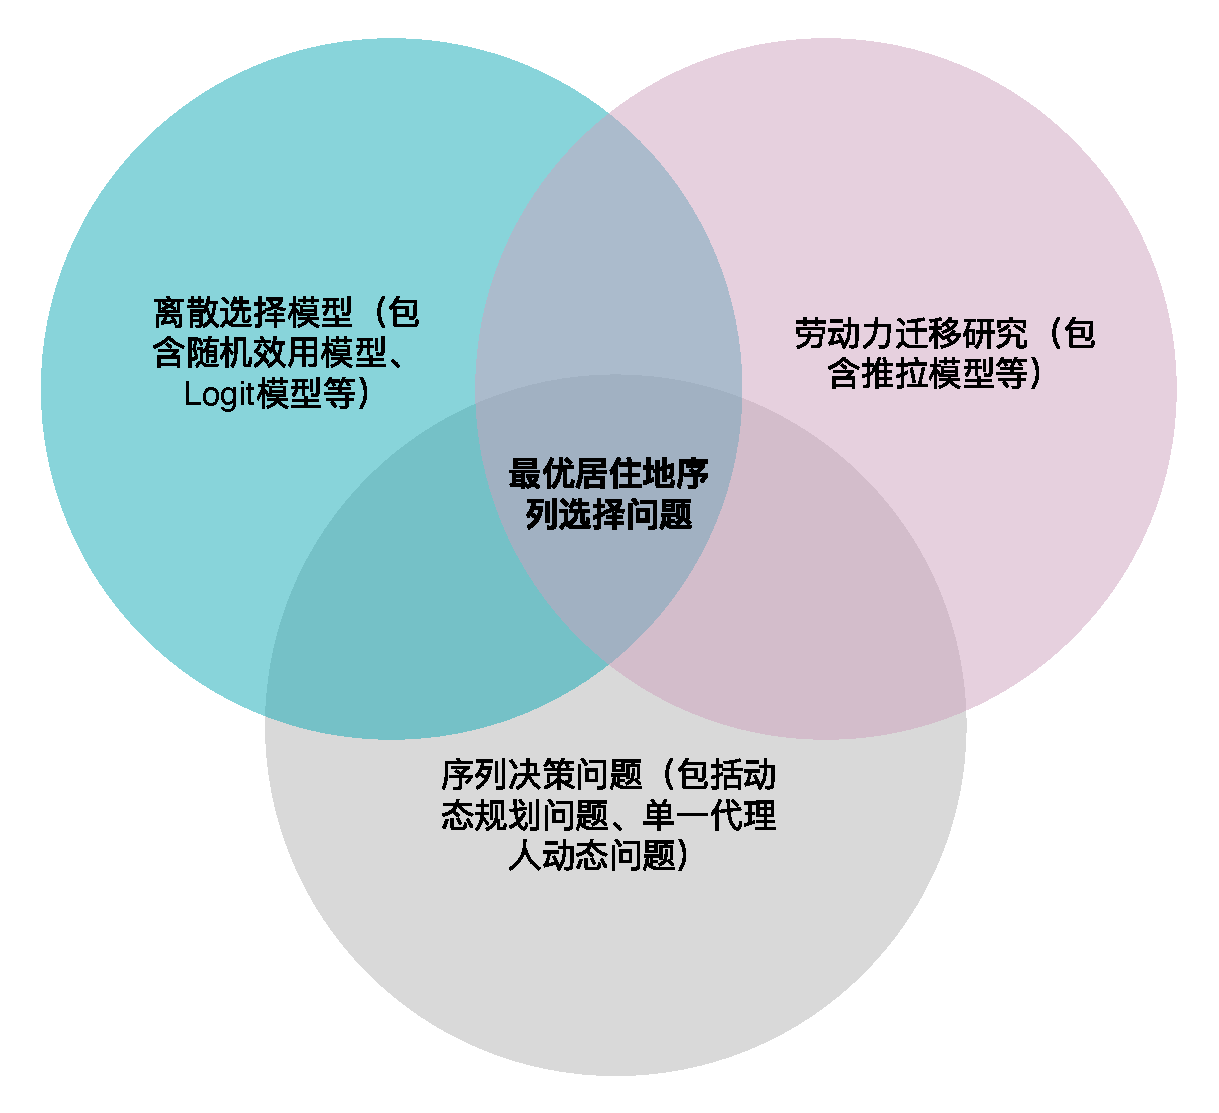
\includegraphics[width=0.65\textwidth]{images/optimal_residential_sequence.drawio.pdf}
\label{fig:最优居住地序列选择问题的理论来源venn diagram}
\end{figure}





















\printbibliography[heading=bibliography,title=参考文献]

\end{document}